%%%%%%%%%%%%%%%%%%%%%%%%%%%%%%%%%%%%%%%%%%%%%%%%%%%%%%%%%%%%%%%%
% %
% Seth Cram %
% ECE351 Section 53 %
% Lab Number 3 %
% Due 02/08/2022 %
% Any other necessary information needed to navigate the file %
%
%
% %
%%%%%%%%%%%%%%%%%%%%%%%%%%%%%%%%%%%%%%%%%%%%%%%%%%%%%%%%%%%%%%%%
%%%%%%%%%%%%%%%%%%%%%%%%%%%%%%%%%%%%%%%%%%%
%%% DOCUMENT PREAMBLE %%%
\documentclass[12pt]{report}
\usepackage[english]{babel}
%\usepackage{natbib}
\usepackage{url}
\usepackage[utf8x]{inputenc}
\usepackage{amsmath}
\usepackage{graphicx}
\graphicspath{{images/}}
\usepackage{parskip}
\usepackage{fancyhdr}
\usepackage{vmargin}
\usepackage{listings}
\usepackage{hyperref}
\usepackage{xcolor}
\usepackage{verbatim}

\definecolor{codegreen}{rgb}{0,0.6,0}
\definecolor{codegray}{rgb}{0.5,0.5,0.5}
\definecolor{codeblue}{rgb}{0,0,0.95}
\definecolor{backcolour}{rgb}{0.95,0.95,0.92}

\begin{comment} %have to use verbatim package for this

\section{Personal Notes}
            


\end{comment}

\lstdefinestyle{mystyle}{
    backgroundcolor=\color{backcolour},   
    commentstyle=\color{codegreen},
    keywordstyle=\color{codeblue},
    numberstyle=\tiny\color{codegray},
    stringstyle=\color{codegreen},
    basicstyle=\ttfamily\footnotesize,
    breakatwhitespace=false,         
    breaklines=true,                 
    captionpos=b,                    
    keepspaces=true,                 
    numbers=left,                    
    numbersep=5pt,                  
    showspaces=false,                
    showstringspaces=false,
    showtabs=false,                  
    tabsize=2
}
 
\lstset{style=mystyle}

\setmarginsrb{3 cm}{2.5 cm}{3 cm}{2.5 cm}{1 cm}{1.5 cm}{1 cm}{1.5 cm}

\title{Lab 4}		%TITLE						
% Title
\author{ Seth Cram}						
% Author
\date{02/15/2022}
% Date

\makeatletter
\let\thetitle\@title
\let\theauthor\@author
\let\thedate\@date
\makeatother

\pagestyle{fancy}
\fancyhf{}
\rhead{\theauthor}
\lhead{\thetitle}
\cfoot{\thepage}
%%%%%%%%%%%%%%%%%%%%%%%%%%%%%%%%%%%%%%%%%%%%
\begin{document}

%%%%%%%%%%%%%%%%%%%%%%%%%%%%%%%%%%%%%%%%%%%%%%%%%%%%%%%%%%%%%%%%%%%%%%%%%%%%%%%%%%%%%%%%%

\begin{titlepage}
	\centering
    \vspace*{0.5 cm}
   % \includegraphics[scale = 0.075]{bsulogo.png}\\[1.0 cm]	% University Logo
\begin{center}    \textsc{\Large   ECE 351 - 53 }\\[2.0 cm]	\end{center}% University Name
	\textsc{\Large System Step Response Using Convolution }\\[.5 cm]				% Course Code
	\rule{\linewidth}{0.2 mm} \\[0.4 cm]
	{ \huge \bfseries \thetitle}\\
	\rule{\linewidth}{0.2 mm} \\[1.5 cm]
	
	\begin{minipage}{0.4\textwidth}
		\begin{flushleft} \large
		%	\emph{Submitted To:}\\
		%	Name\\
          % Affiliation\\
           %contact info\\
			\end{flushleft}
			\end{minipage}~
			\begin{minipage}{0.4\textwidth}
            
			\begin{flushright} \large
			\emph{Submitted By :} \\
			Seth Cram  
		\end{flushright}
           
	\end{minipage}\\[2 cm]
	
\end{titlepage}

%%%%%%%%%%%%%%%%%%%%%%%%%%%%%%%%%%%%%%%%%%%%%%%%%%%%%%%%%%%%%%%%%%%%%%%%%%%%%%%%%%%%%%%%%

\tableofcontents
\pagebreak

%%%%%%%%%%%%%%%%%%%%%%%%%%%%%%%%%%%%%%%%%%%%%%%%%%%%%%%%%%%%%%%%%%%%%%%%%%%%%%%%%%%%%%%%%
\renewcommand{\thesection}{\arabic{section}}

\section{Introduction}

The goal of lab 4 is to become even more familiar with convolution by computing a system's step response using Python in the Spyder IDE.

\section{Equations}
    \begin{equation*}
        u(t) = \{t<0:0, t>=0:1\}
    \end{equation*}
 
    \begin{equation*}
        h_1(t) = e^{-2t} \cdot [u(t) - u(t-3)]
    \end{equation*}
    
    \begin{equation*}
        h_2(t) = u(t − 2) − u(t − 6)
    \end{equation*}
    
    \begin{equation*}
        h_3(t) = cos( w_0t ) \cdot u(t)
    \end{equation*}
    
    \begin{equation*}
        w_0 = F_0 \cdot 2 \cdot \pi
    \end{equation*}

    \begin{equation*}
        h_1(t) * u(t) = 0.5 \cdot (-e^{-2t} + 1) \cdot u(t) - 0.5 \cdot (-e^{-2(t-3)}+1) \cdot u(t-3)
    \end{equation*}
    
    \begin{equation*}
        h_2(t) * u(t) = (t-2) \cdot u(t-2) - (t-6) \cdot u(t-6)
    \end{equation*}
    
    \begin{equation*}
        h_3(t) * u(t) = 0.63662 \cdot sin(1.5708t) \cdot u(t)
    \end{equation*}
    
    \begin{center} or \end{center}
    \begin{equation*}
        h_3(t) * u(t) = 1/w_0 \cdot sin(w_0t) \cdot u(t)
    \end{equation*}
    
\section{Methodology}

%This section will describe how you went about solving the lab. Make sure you go into detail about any method you used. %Include coding samples here if necessary. This is also where you would include necessary derivations. An example of %inserting code into the report is given. Do not go overboard on inserting code into your report, only use whats %absolutely necessary to illustrate your point.

    \paragraph{} I began by creating a new file to house just my convolution function. Within my main file for project 3, I imported the convolution, step, and ramp functions. I got the step and ramp functions from the previous project. From there, it was easy to create the h1-3 functions and plot them.  

    \paragraph{} Now, it was time to plot the step response using the convolution function we'd built. I made sure to double the number of t-values after convolving, so the convolved function could be plotted. I doubled the number of t-values by halving the step size. Realizing how long my convolution function took to solve, I decided to use the library convolution function. The TA clarified that it'd be okay to do so, and I'm grateful because of how slow our user-defined convolution through summation is.      
    
    \paragraph{} Calculating out the step response to the convolution functions by hand was relatively simple since we'd already taken the exam for convolution. Regardless, I was grateful to our TA for walking through the process to make sure we knew we had the correct results and were going about solving the convolution properly. 
    
\section{Results}

%This section will go over the results of the lab. Use this area to describe %if the lab worked as expected or if the results are unexpected or different %from your hand calculations or intuition. Part of being a good engineer is %gaining intuition about these problems and being able to understand quickly %if something is wrong. Use code, plots, tables, and figures as necessary. %Make sure to cite all other works used and note them in the bibliography. A %sample entry is in this document.

    \paragraph{} As mentioned above, after creating the h1-3 functions, I plotted them together on a single figure. I expected an exponential function starting at 1, a rectangular wave from 2 to 6, and a sinusoidal curve starting at zero.

    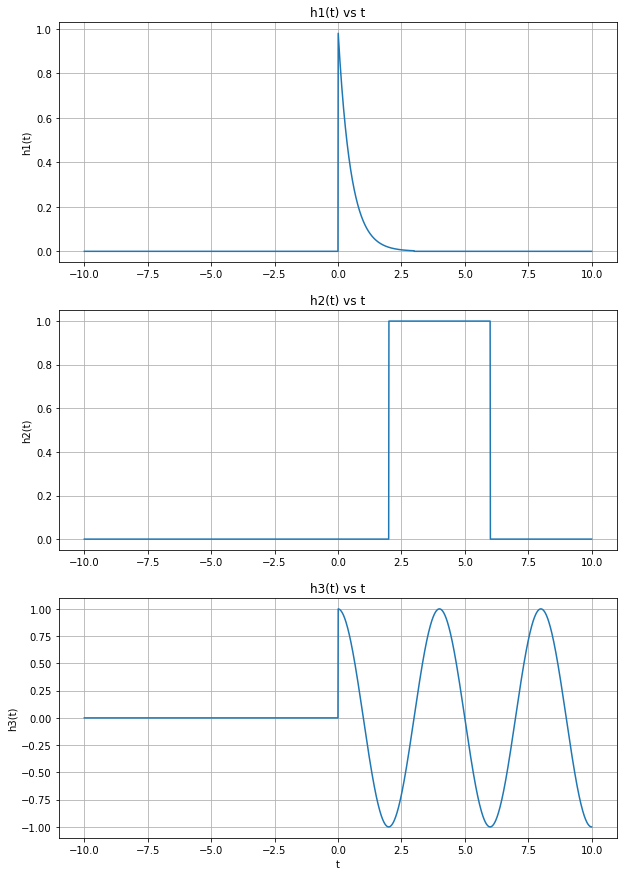
\includegraphics[scale=0.6]{functs h1-3.png}

    \paragraph{} As seen above, most of my expectations held true with the exception of the first function. Instead, the first function started at 0 and near 2.5.    
    
    \paragraph{} I used the library's convolve function to plot the step response to functions h1-3. I plotted them together on a single figure for easy comparison, to when I plot the hand-calculated step response of the functions. I expected the first function to be much more curved, the second one to have shallower slopes, and the third one to be smoother. 
    
    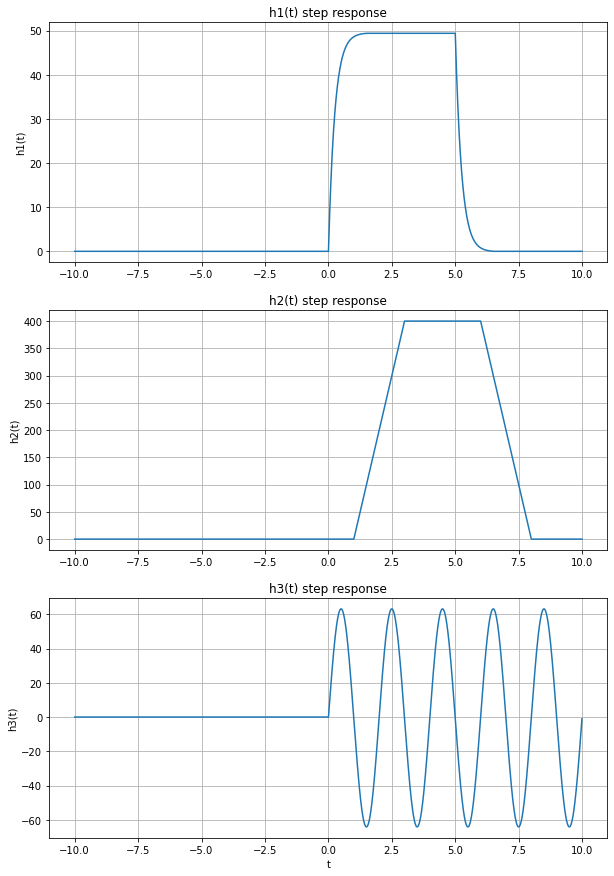
\includegraphics[scale=0.6]{h1-3 funct response.png}
    
    \paragraph{} I didn't predict the shape of the first function whatsoever, but was somewhat correct. My expectation was dead on for the second function. Although, I didn't expect the third function to attain a smaller period. 
    
    \paragraph{} As seen in the Equations section, I hand-convolved the given functions. Just to reiterate, I'll list them down here as well. 
    
    \begin{equation*}
        h_1(t) * u(t) = 0.5 \cdot (-e^{-2t} + 1) \cdot u(t) - 0.5 \cdot (-e^{-2(t-3)}+1) \cdot u(t-3)
    \end{equation*}
    
    \begin{equation*}
        h_2(t) * u(t) = (t-2) \cdot u(t-2) - (t-6) \cdot u(t-6)
    \end{equation*}
    
    \begin{equation*}
        h_3(t) * u(t) = 0.63662 \cdot sin(1.5708t) \cdot u(t)
    \end{equation*}
    
    \begin{center} or \end{center}
    \begin{equation*}
        h_3(t) * u(t) = 1/w_0 \cdot sin(w_0t) \cdot u(t)
    \end{equation*}
    
    \paragraph{} Despite how much convolution I've already done, I didn't expect the resultant step response of any of the three functions beforehand. Moving onto plotting these, I expected the plots to line up perfectly with those from the library's convolution function.  
    
    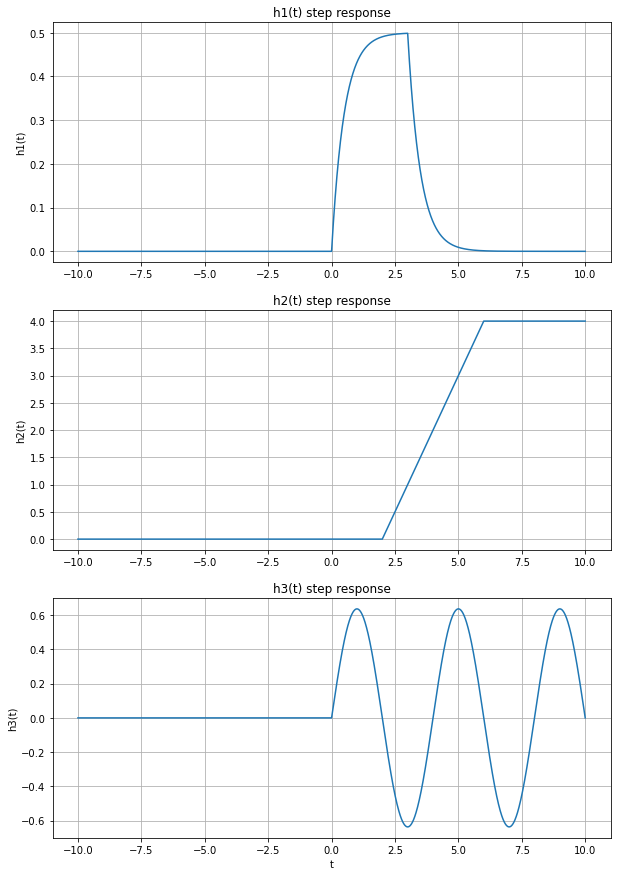
\includegraphics[scale=0.6]{h1-3 hand response.png}
    
    \paragraph{} As seen above, the convolved functions are completely different from before. This is especially prevalent when comparing the y-axis. For whatever reason, convolution through integration gave us much larger values than convolution through summation. They also resulted in different overall shapes.  
      

\section{Error Analysis}

%This section will discuss error analysis of the experiment. Since this lab %deals with ideal simulation there shouldn't be any sources of error, so %instead this section can be used to describe any difficulties you had during %lab and how you solved them. Alternatively, if you couldn't get the %experiment to work, which is okay, you need to use this section to explain why %you couldn't get it to work to earn full points. 

\paragraph{} A possible form of error includes: not plotting the full breadth of the second convolved function when done with integration. It's entirely possible that the function eventually falls back down to zero like its summation counterpart and we just didn't plot for a wide enough range of values. This could result in an incorrect comparison of function two's convolved function shape resulting from integration.  

\section{Questions} %also address any deliverables not yet put in yet
    \begin{enumerate}
        \item Leave any feedback on the clarity of lab tasks, expectations, and deliverables
        \paragraph{} A part of the lab that confused me was that it said in the lab handout that our hand-calculated functions and the Python generated ones were supposed to have matching plots. This was not the case. 
    \end{enumerate}

\section{Conclusion}

%Discuss briefly what you learned in this lab and whether or not you feel the %lab was successful. Include any recommendations for future labs as this is a %learning experience for all of us. Discuss any insights you gained from this %lab and how that will affect future work. \textit{Note: The bibliograhpy %needs to be on its own page.}

    \paragraph{} From lab 4, I learned that convolving functions through summation or integration resulted in different results. It helped me realize the limits of summation, even when a computer is using it. Overall, I feel like this lab was successful since it introduced me to using convolution to find a system's step response and the differences between summation and integration convolution. 

Github: \url{https://github.com/SethCram} 

\newpage

\end{document}